%!TEX root =../mapp-challenge-18-game-book.tex
% ^ leave for LaTeXTools build functionality

\phChapterWorksheet{Knot True}{Teaser Puzzle}

In \phEventName{}, your team will travel to the world of
\textbf{\mappMobimon{}}, where trainers befriend monsters and battle them
against their opponents!
(Now where have I heard that idea before?...) Of course, you'll probably
find yourself encountering a wild \textbf{puzzle} or two, so let's see how
you deal with this conundrum...

In a previous \mappMobimon{} tournament, six trainers competed and were
ranked 1st through 6th: Ash, Brock, Cynthia, Drayden, Erika, and Flannery.
You have been told the following facts about these results:

\begin{multicols}{3}\footnotesize
  \begin{center}
    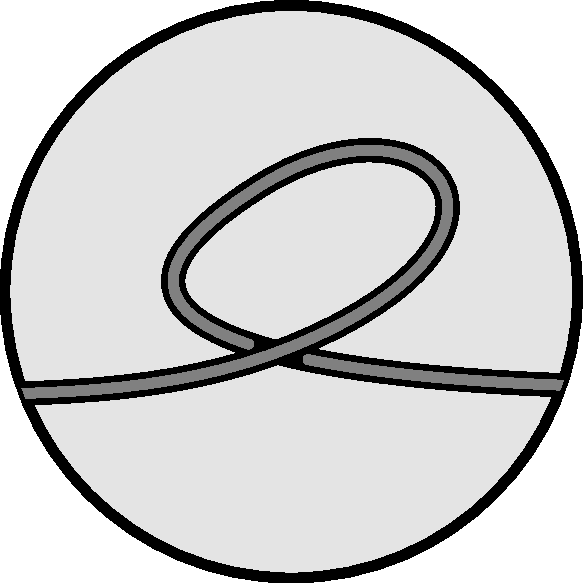
\includegraphics[width=1.2in]{assets/unknot1.pdf}

    Ash and Flannery did not place 6th.


    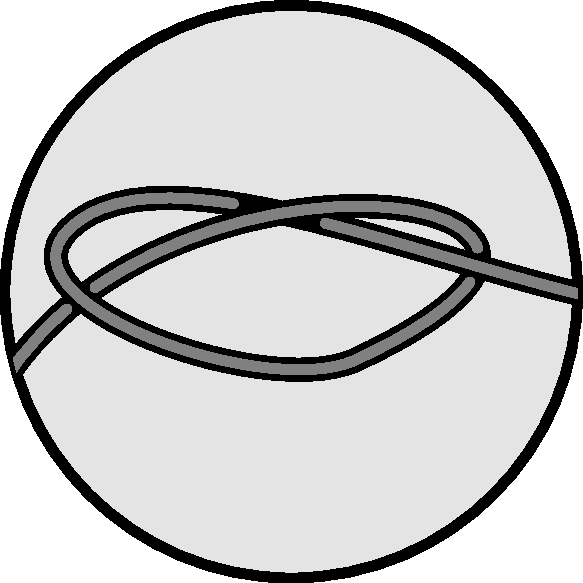
\includegraphics[width=1.2in]{assets/knot1.pdf}

    Neither Brock nor Drayden placed 4th.


    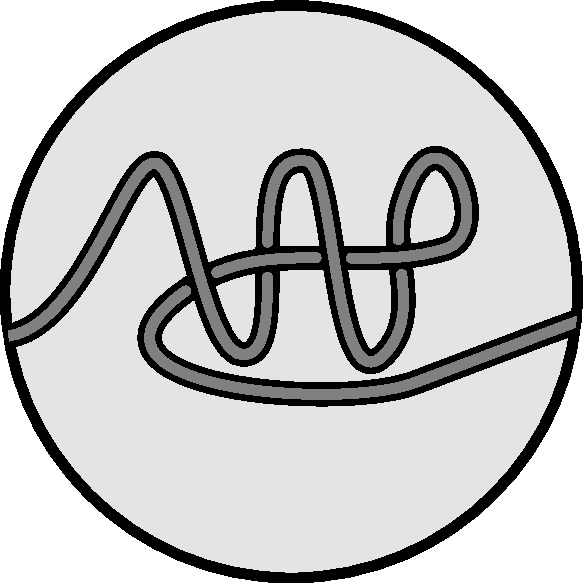
\includegraphics[width=1.2in]{assets/unknot2.pdf}

    Erika placed exactly one rank higher than Ash.


    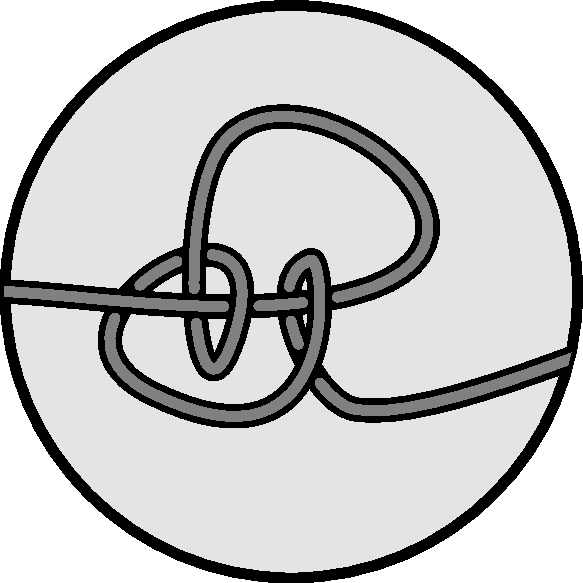
\includegraphics[width=1.2in]{assets/knot2.pdf}

    Drayden placed in the top three.


    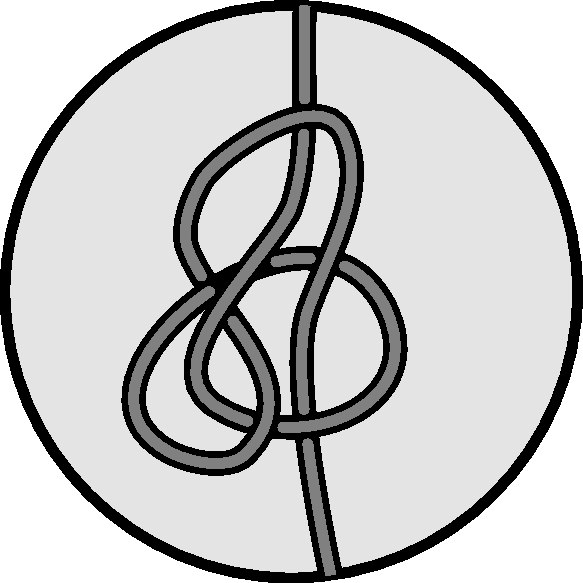
\includegraphics[width=1.2in]{assets/knot3.pdf}

    Brock placed lower than Flannery.


    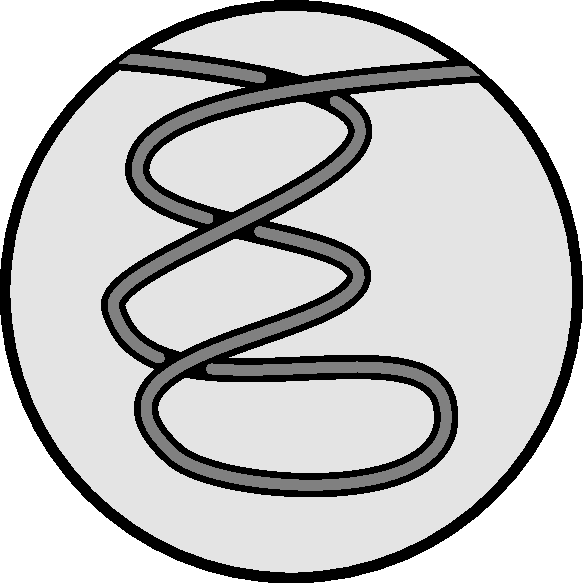
\includegraphics[width=1.2in]{assets/unknot3.pdf}

    Either Cynthia or Drayden placed 3rd.
  \end{center}
\end{multicols}

Unfortunately, there's no way all of those claims are \textbf{truthful}.
By inspecting the \textbf{Trainer Badge} above each statement, you can uncover
the \textbf{lies} by deciding if the cord depicted in its design would
\textbf{tighten into a knot} if pulled taut. By blacking out the incorrect
results below, you'll reveal the answer to this riddle: \textit{what is a
mathematician's favorite kind of knot?}

\begin{center}\footnotesize
\begin{tikzpicture}[x=0.2in,y=0.2in]
  \draw[thick] (0,0) rectangle (6,6);
  \draw[step=1] (0,0) grid (6,6);
  \node[anchor=south] at (0.5,6) {\rotatebox{90}{Ash}};
  \node[anchor=south] at (1.5,6) {\rotatebox{90}{Brock}};
  \node[anchor=south] at (2.5,6) {\rotatebox{90}{Cynthia}};
  \node[anchor=south] at (3.5,6) {\rotatebox{90}{Drayden}};
  \node[anchor=south] at (4.5,6) {\rotatebox{90}{Erika}};
  \node[anchor=south] at (5.5,6) {\rotatebox{90}{Flannery}};
  \node[anchor=east] at (0,5.5) {1st};
  \node[anchor=east] at (0,4.5) {2nd};
  \node[anchor=east] at (0,3.5) {3rd};
  \node[anchor=east] at (0,2.5) {4th};
  \node[anchor=east] at (0,1.5) {5th};
  \node[anchor=east] at (0,0.5) {6th};
  \foreach \letters [count=\i] in {
    {O,Y,G,U,S,J},
    {Q,C,M,V,A,X},
    {F,P,U,N,I,E},
    {L,A,S,I,D,T},
    {K,N,B,Z,T,R},
    {H,R,W,E,L,M},
  } {
    \foreach \letter [count=\j] in \letters {
      \node at ($(\j.5,-\i.5)+(-1,7)$) {\letter};
    }
  }
\end{tikzpicture}
\end{center}


\phWorksheet{Teaser Puzzle Solution}

The following cords wouldn't tighten into a knot, so their clues are
\textbf{true}.

\begin{multicols}{3}\footnotesize
  \begin{center}
    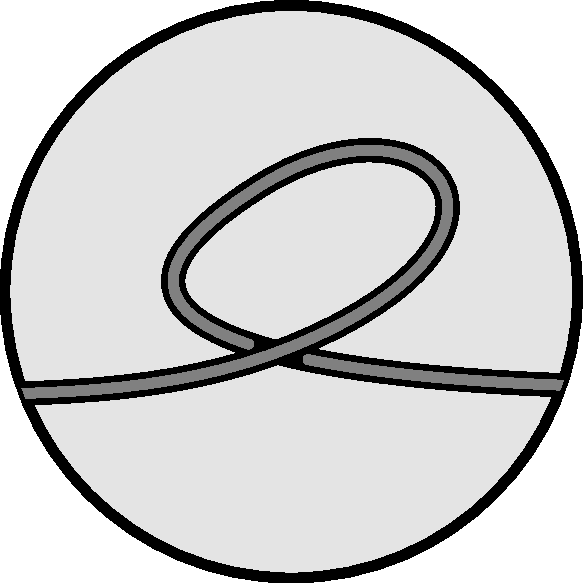
\includegraphics[width=1.2in]{assets/unknot1.pdf}

    Ash and Flannery did not place 6th.


    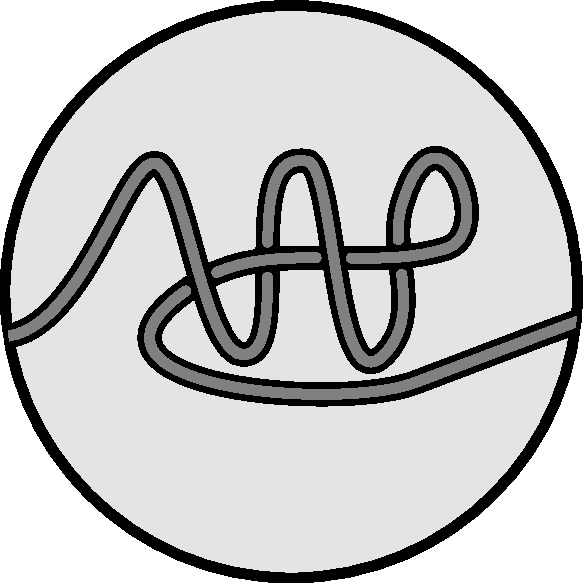
\includegraphics[width=1.2in]{assets/unknot2.pdf}

    Erika placed exactly one rank higher than Ash.


    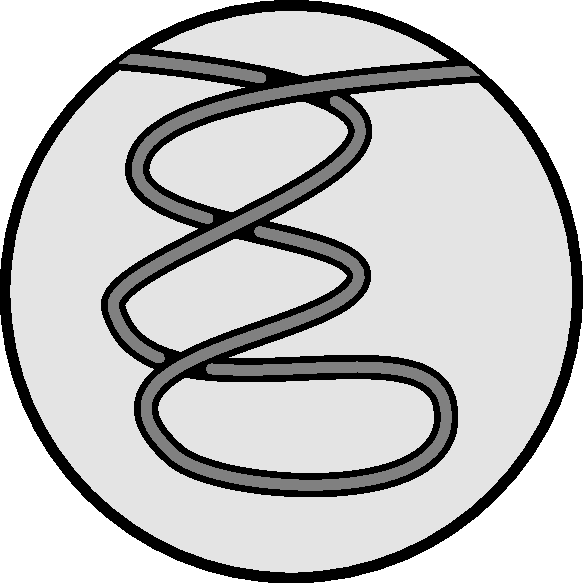
\includegraphics[width=1.2in]{assets/unknot3.pdf}

    Either Cynthia or Drayden placed 3rd.
  \end{center}
\end{multicols}

The following cords would tighten into a knot, so their clues are
\textbf{false}.

\begin{multicols}{3}\footnotesize
  \begin{center}
    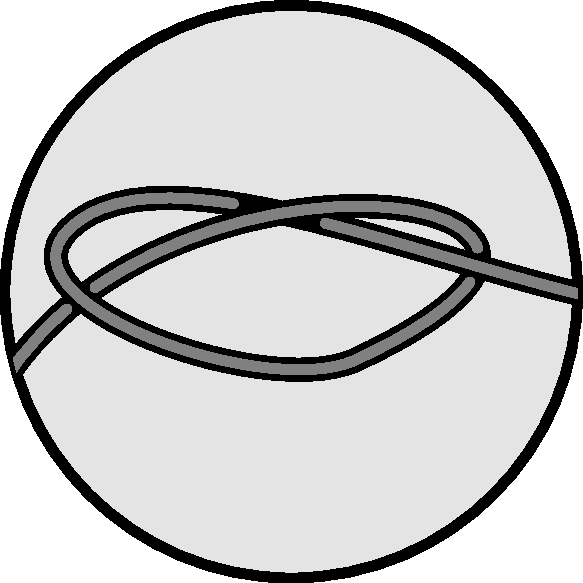
\includegraphics[width=1.2in]{assets/knot1.pdf}

    \textit{Neither Brock nor Drayden placed 4th.}
    Corrected: Either Brock or Drayden placed 4th.


    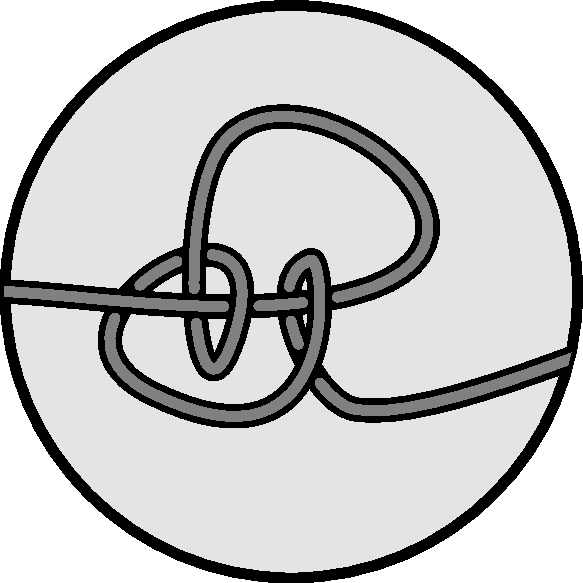
\includegraphics[width=1.2in]{assets/knot2.pdf}

    \textit{Drayden placed in the top three.}
    Corrected: Drayden placed in the bottom three.


    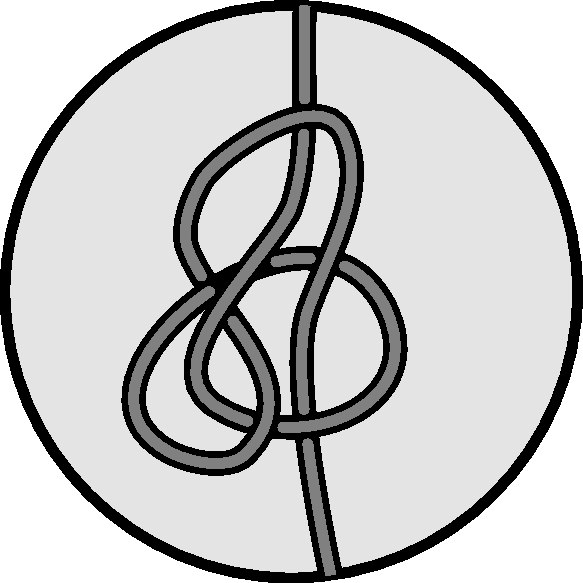
\includegraphics[width=1.2in]{assets/knot3.pdf}

    \textit{Brock placed lower than Flannery.}
    Corrected: Brock placed higher than Flannery.
  \end{center}
\end{multicols}

Logically, this results in the following grid.

\begin{center}\footnotesize
\begin{tikzpicture}[x=0.2in,y=0.2in]
  \draw[thick,fill=black!80] (0,0) rectangle (6,6);
  \draw[step=1] (0,0) grid (6,6);
  \node[anchor=south] at (0.5,6) {\rotatebox{90}{Ash}};
  \node[anchor=south] at (1.5,6) {\rotatebox{90}{Brock}};
  \node[anchor=south] at (2.5,6) {\rotatebox{90}{Cynthia}};
  \node[anchor=south] at (3.5,6) {\rotatebox{90}{Drayden}};
  \node[anchor=south] at (4.5,6) {\rotatebox{90}{Erika}};
  \node[anchor=south] at (5.5,6) {\rotatebox{90}{Flannery}};
  \node[anchor=east] at (0,5.5) {1st};
  \node[anchor=east] at (0,4.5) {2nd};
  \node[anchor=east] at (0,3.5) {3rd};
  \node[anchor=east] at (0,2.5) {4th};
  \node[anchor=east] at (0,1.5) {5th};
  \node[anchor=east] at (0,0.5) {6th};
  \foreach \letters [count=\i] in {
    {O,Y,G,U,S,J},
    {Q,C,M,V,A,X},
    {F,P,U,N,I,E},
    {L,A,S,I,D,T},
    {K,N,B,Z,T,R},
    {H,R,W,E,L,M},
  } {
    \foreach \letter [count=\j] in \letters {
      \node at ($(\j.5,-\i.5)+(-1,7)$) {\letter};
    }
  }
  \node[circle,inner sep=2pt,draw,fill=white] at (4.5,5.5) {S};
  \node[circle,inner sep=2pt,draw,fill=white] at (0.5,4.5) {Q};
  \node[circle,inner sep=2pt,draw,fill=white] at (2.5,3.5) {U};
  \node[circle,inner sep=2pt,draw,fill=white] at (1.5,2.5) {A};
  \node[circle,inner sep=2pt,draw,fill=white] at (5.5,1.5) {R};
  \node[circle,inner sep=2pt,draw,fill=white] at (3.5,0.5) {E};
\end{tikzpicture}
\end{center}

A mathematican's favorite knot is a \texttt{SQUARE} knot! Oh... you say
you've heard that one before? Well, our \textbf{puzzles} are better than our \textbf{jokes} at the \textbf{MaPP Challenge}, so we hope to see you there!


% Include below for aucTeX integration
%%% Local Variables:
%%% mode: latex
%%% TeX-master: "../mapp-challenge-18-game-book"
%%% End:
